% ==============================================================================
\section{Introduction}
Computer vision is a field that has grown explosively in the last few years, very much in thanks to the utilization of Convolutional Neural Networks, or CNN's, to accurately identify different kinds of information from raw image data. This capability has led to many different subfields of research, including 3D localization of objects using a variety of sensor setups. To that end, a few questions naturally arise: how many sensors are needed to accurately locate objects, and what trade-offs exist for using more or less sensors?

To that end, a paper is proposed to seek out a comparison between two specific sensor setups. The first sensor setup would use only camera data, and a derived stereo disparity image, to detect and localize the desired object of interest, specifically cars. The second sensor setup would use a single camera and a single lidar to perform the same task. The nature of the detection required would be a 3D bounding box, expressed as a box with real-world distances to describe an object's relative x, y, and z coordinates as well as its height, width, and length. The dataset that would be used for this task is not yet confirmed, but is currently one out of several possibilities, described below. Each of these possible datasets will be expanded upon below, describing their merits and drawbacks.

% ==============================================================================
\section{Literature Search Questions}
There are multiple questions to answer regarding what is possible in this project. To that end, a literature search is underway to answer:

\begin{itemize} \itemsep=-0.5em
\item What is the state of the art in current stereo vision-based object detection?
\item What is the state of the art in current camera/lidar-based object detection?
\item What dataset meets the required criteria for usage in this project?
\item How are 3D bounding boxes evaluated, and what standard is used to obtain a score, such as precision, recall, and average precision?
\end{itemize}

% ==============================================================================
\subsection{State of the Art: Stereo-Based Object Detection}
To know the state of the art (SOTA) of stereo-based object detection, 

\subsection{State of the Art: Camera/Lidar-Based Object Detection}
TextHere

\subsection{Valid Datasets, and the Most Qualified to be Used}
In order to perform good object detection, a dataset must exist that meets the project needs. In this project, the various requirements are listed below. \\

A usable dataset for this project must have: 
\begin{itemize} \itemsep=-0.5em
    \item RGB (red/green/blue, 3-channel) images
    \item Stereo vision disparity maps, or the ability to generate them
    \item Man-made objects as the class of interest, e.g. cars
    \item 3D bounding boxes for object localization
    \item Data collected in an outside setting
    \item OPTIONAL: lidar data containing the class of interest (for future comparison with other methods).
\end{itemize}

Based on these criteria, some datasets may be valid or invalid, and merit investigation. The following datasets all meet the necessary requirements, and some also contain the optional requirement.
\begin{itemize} \itemsep=-0.5em
    \item The KITTI dataset (3D detection task)
    \item Oxford RobotCar dataset (3D detection task)
    \item Berkeley DeepDrive Dataset
    \item (TBD)
\end{itemize}


\subsection{3D Bounding Box Evaluation}
TextHere

\section{Project Schedule / Timeline}
In order to meet all requirements while also satisfying educational program requirements, a proposed timeline is provided below. Notable dates here include the official start of the thesis, the final date of the thesis, including presentation and document turn-in.

% kjgnote: "makebox" used in order to make an oversized-but-still-centered figure
\begin{figure}[h] % ahh, h = "approx here", t = "top of page", b = "bottom of pg"
    \makebox[\textwidth][c]{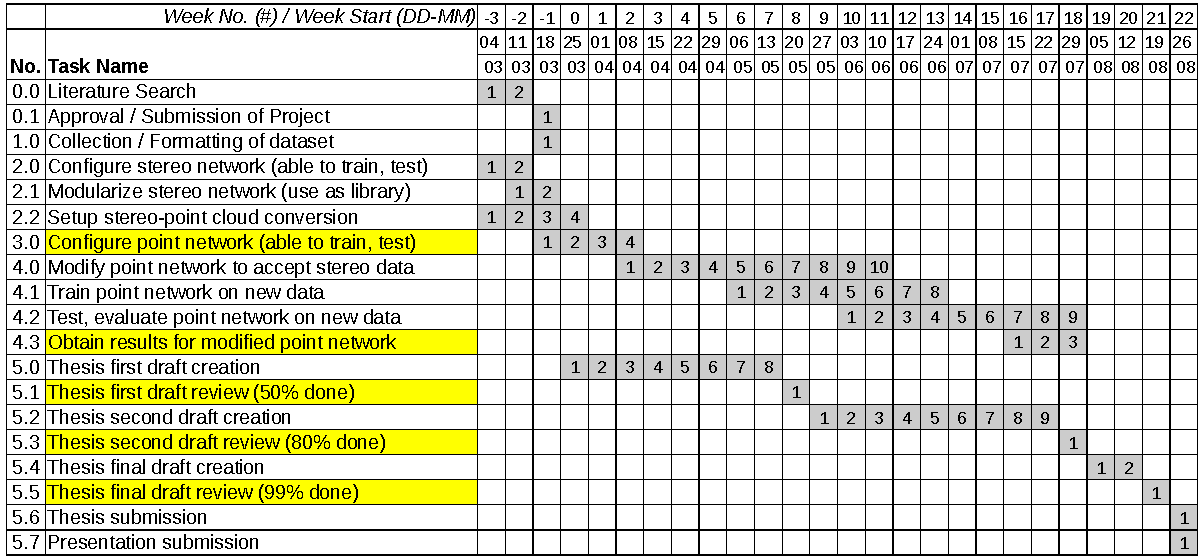
\includegraphics[scale=.6]{m/proposed_timeline.pdf}}
    \caption{Proposed schedule of paper. Highlighted tasks are critical milestones. Numbers inside of gray cells indicate the number of weeks each individual task lasts.}
% \label{figure-parking}
\end{figure}


\subsection{Same Problem but Different Solution}
Lorem ipsum dolor sit amet, consetetur sadipscing elitr, At accusam aliquyam diam diam dolore dolores duo eirmod eos erat, et nonumy sed tempor et et invidunt justo labore Stet clita ea et gubergren, kasd magna no rebum. sanctus sea sed takimata ut vero voluptua. est Lorem ipsum dolor sit amet. Lorem ipsum dolor sit amet, consetetur\\
\section{Conclusion}
 Lorem ipsum dolor sit amet, consectetur adipiscing elit. Curabitur augue dui, lacinia quis gravida sit amet, dignissim at justo. Pellentesque posuere, tellus id facilisis iaculis, purus nisi convallis purus, in dignissim risus sapien porta velit. Vivamus mauris lorem, facilisis eget luctus eu, sagittis sed erat. Suspendisse pulvinar semper feugiat. Praesent interdum magna orci, molestie efficitur nisi finibus vel. Vestibulum ut porta nibh, non condimentum nisl.
